% Source: https://github.com/rodgzilla/talk-slides/blob/master/deep_learning/transformer_language_model/figures/language_modeling.tex
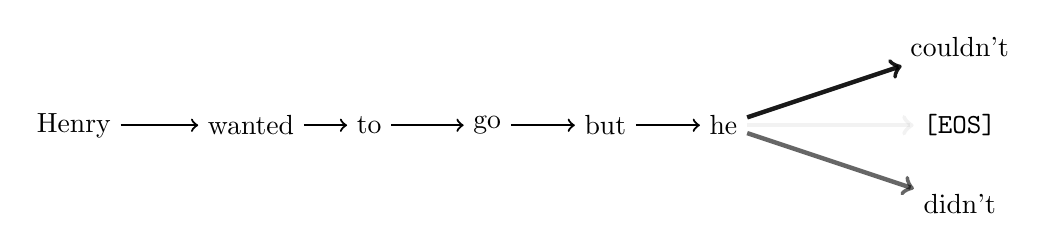
\begin{tikzpicture}[xscale = 1.5]
    \node (W1) at (-.5, 0) {
      Henry
    };
  
  
    \node (W2) at (1, 0) {
      wanted
    };
  
    \node (W3) at (2, 0) {
      to
    };
  
    \node (W4) at (3, 0) {
      go
    };
  
    \node (W5) at (4, 0) {
      but
    };
  
    \node (W6) at (5, 0) {
      he
    };
  
    \node (W8) at (7, 1) {
      couldn't
    };
  
    \node (W9) at (7, 0) {
      \texttt{[EOS]}
    };
  
    \node (W10) at (7, -1) {
      didn't
    };
  
    \draw[thick, ->] (W1) -- (W2);
    \draw[thick, ->] (W2) -- (W3);
    \draw[thick, ->] (W3) -- (W4);
    \draw[thick, ->] (W4) -- (W5);
    \draw[thick, ->] (W5) -- (W6);
    \draw[ultra thick, ->, opacity = 0.9] (W6) -- (W8);
    \draw[ultra thick, ->, opacity = 0.05] (W6) -- (W9);
    \draw[ultra thick, ->, opacity = 0.6] (W6) -- (W10);
  \end{tikzpicture}
